%!TEX root = ../dissertation.tex

\chapter{Implementation}
\label{chapter:implementation}
Chapter~\ref{chapter:implementation} describes the implementation details for the solution that was
presented in the previous chapter. Here we described the technological components of our smart
warehouse for the proposed solution, as well we describe the implementation and technological details
for the provisioning mechanism.

% Smart Warehouse Deployment
\section{Smart Warehouse Deployment}
\label{sec:Smart Place}
The smart warehouse setup was based in a real scenario described by Correia et al. \cite{correiaalpharfid},
as illustrated in Figure~\ref{fig:rfidapp_setup}.\\

% RFID application setup
\begin{figure}[ht!]
  \centering
  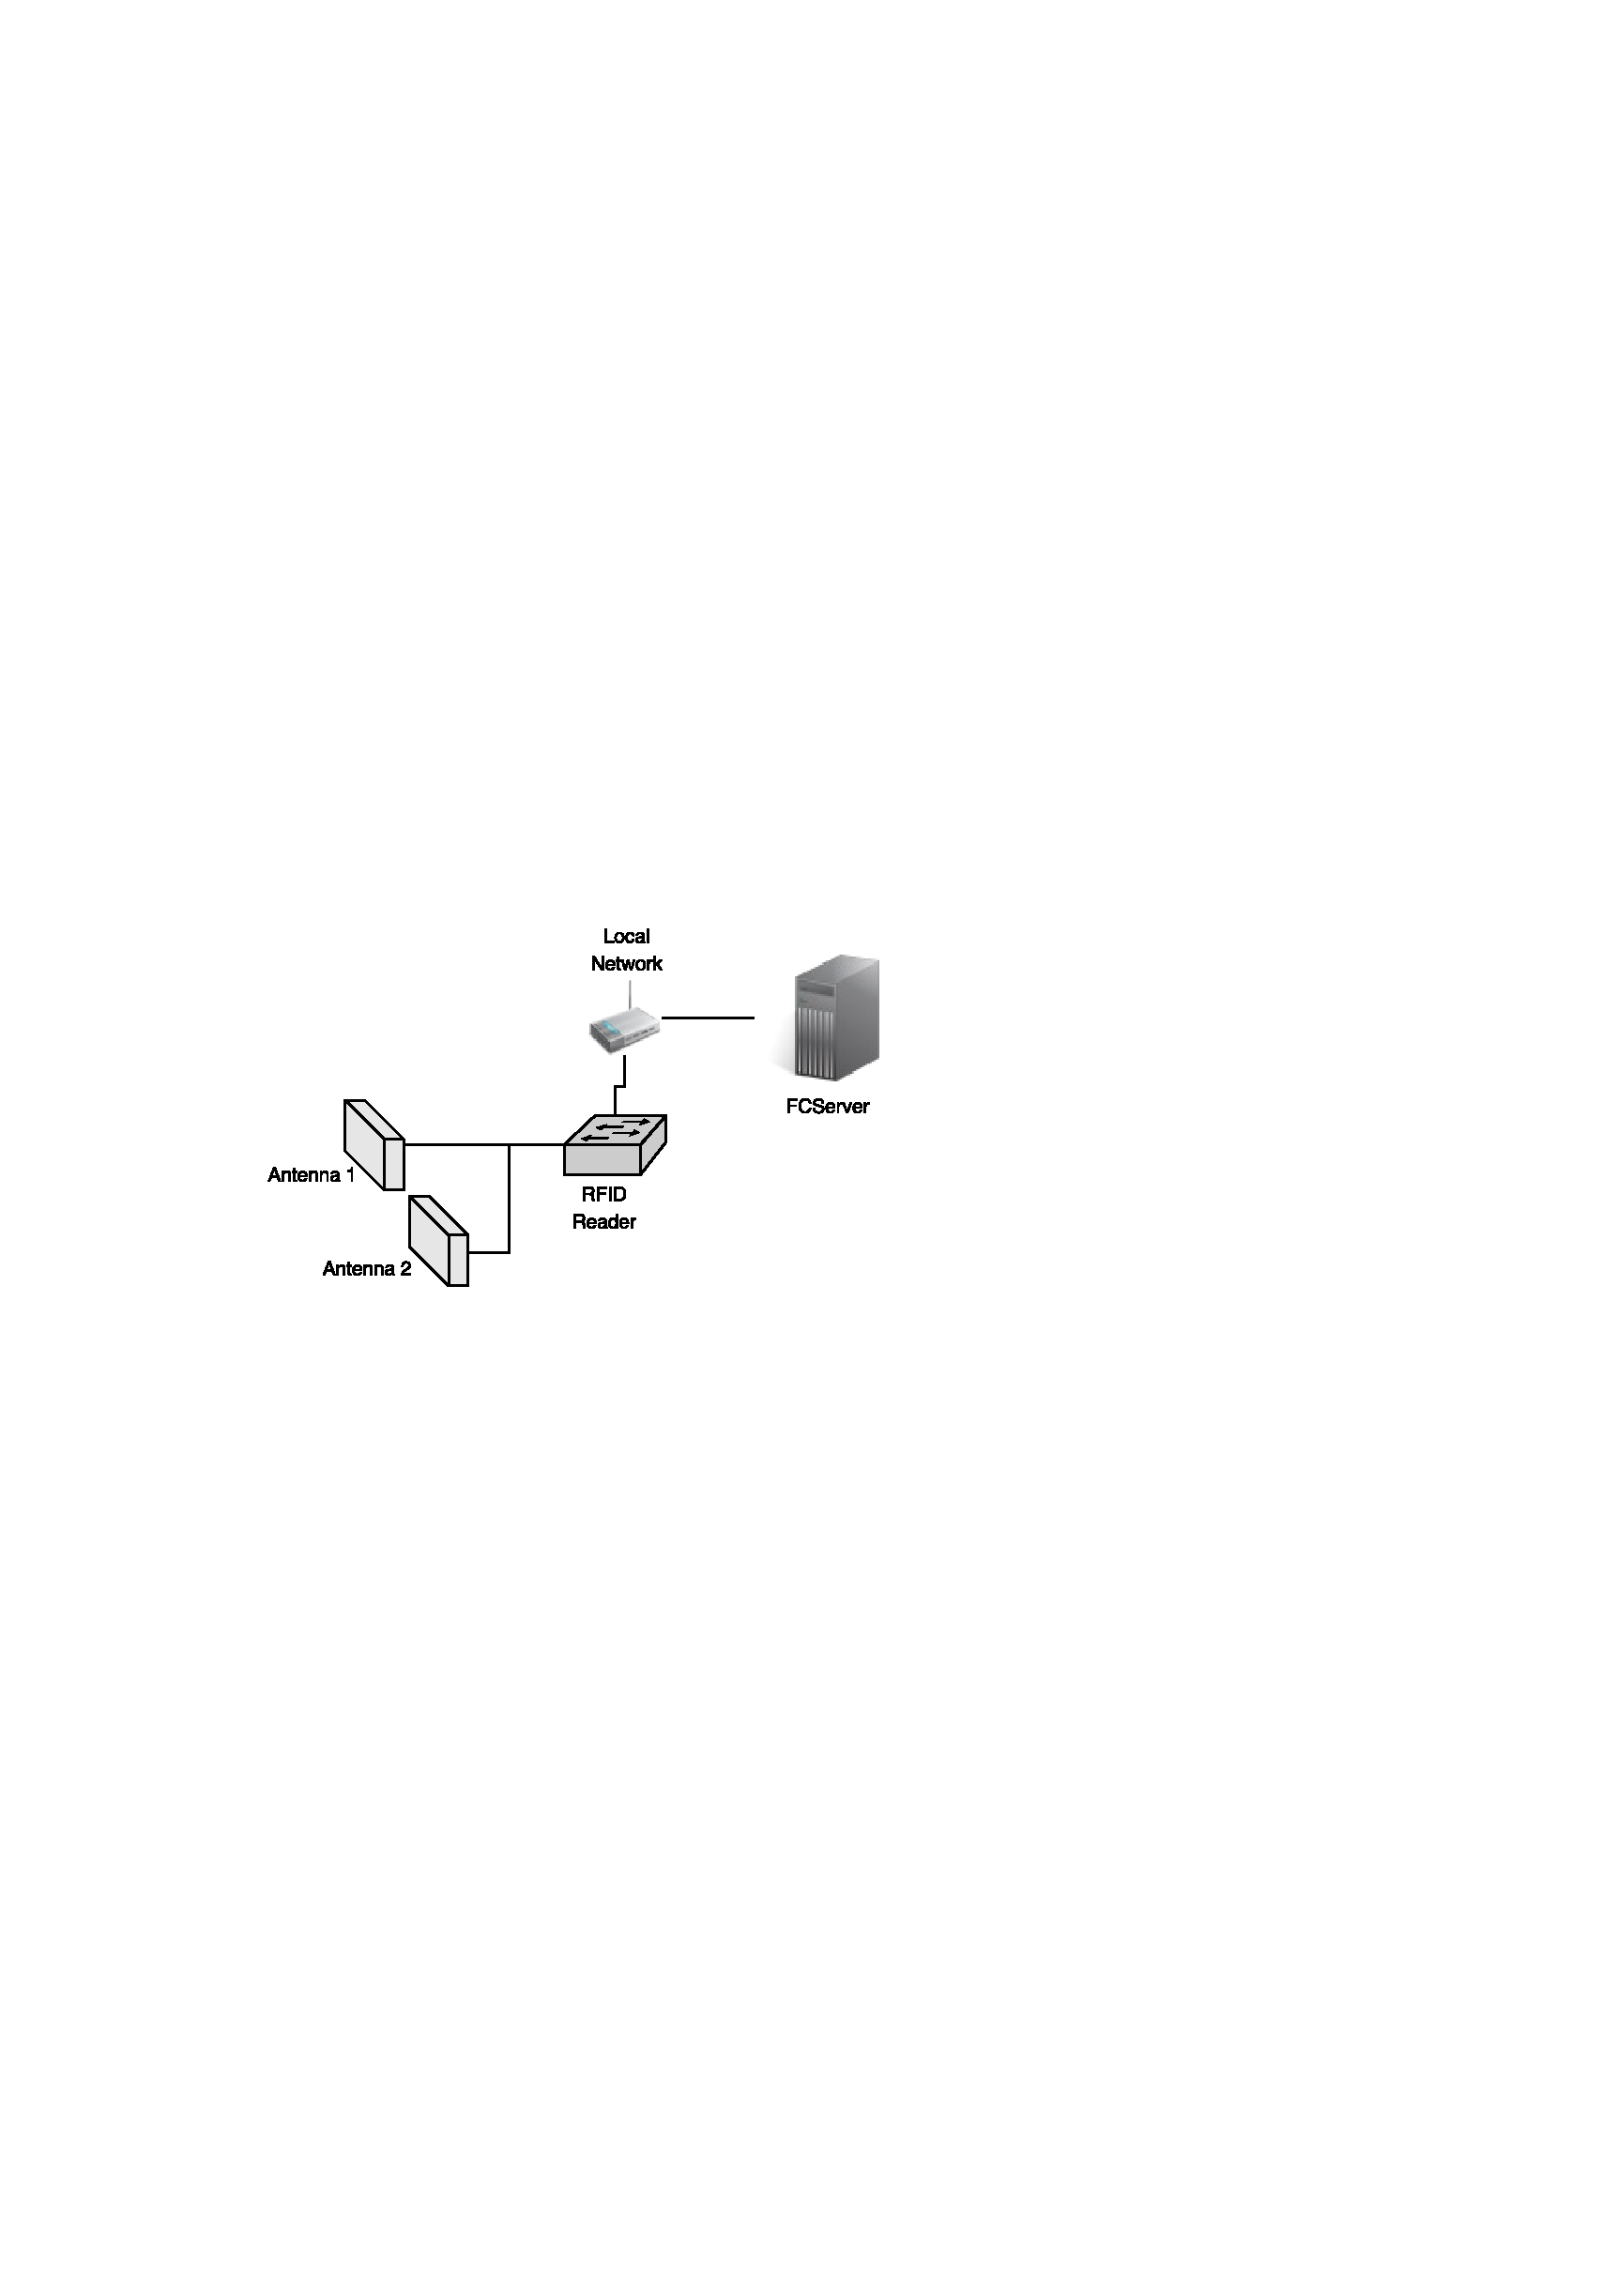
\includegraphics[width=.6\textwidth]{./images/rfidapp_setup}
  \caption[RFID application setup.]{RFID application setup.}
  \label{fig:rfidapp_setup}
\end{figure}

The warehouse is composed of a tagged robot that is identified by \gls{RFID} readers that are deployed
in the physical space. To monitoring the robot inside the warehouse, we decide to use the Fosstrak
platform as our \gls{RFID} middleware. In our implementation, the \gls{RFID} readers are emulated
through the Rifidi Emulator, which uses the \gls{LLRP} protocol to communicate with the Fosstrak
platform.

% Cloud approach
\subsection{Cloud Deployment}
\label{sub:imp_smart_warehouse_cloud}

% Cloud approach
\begin{figure}
  \centering
  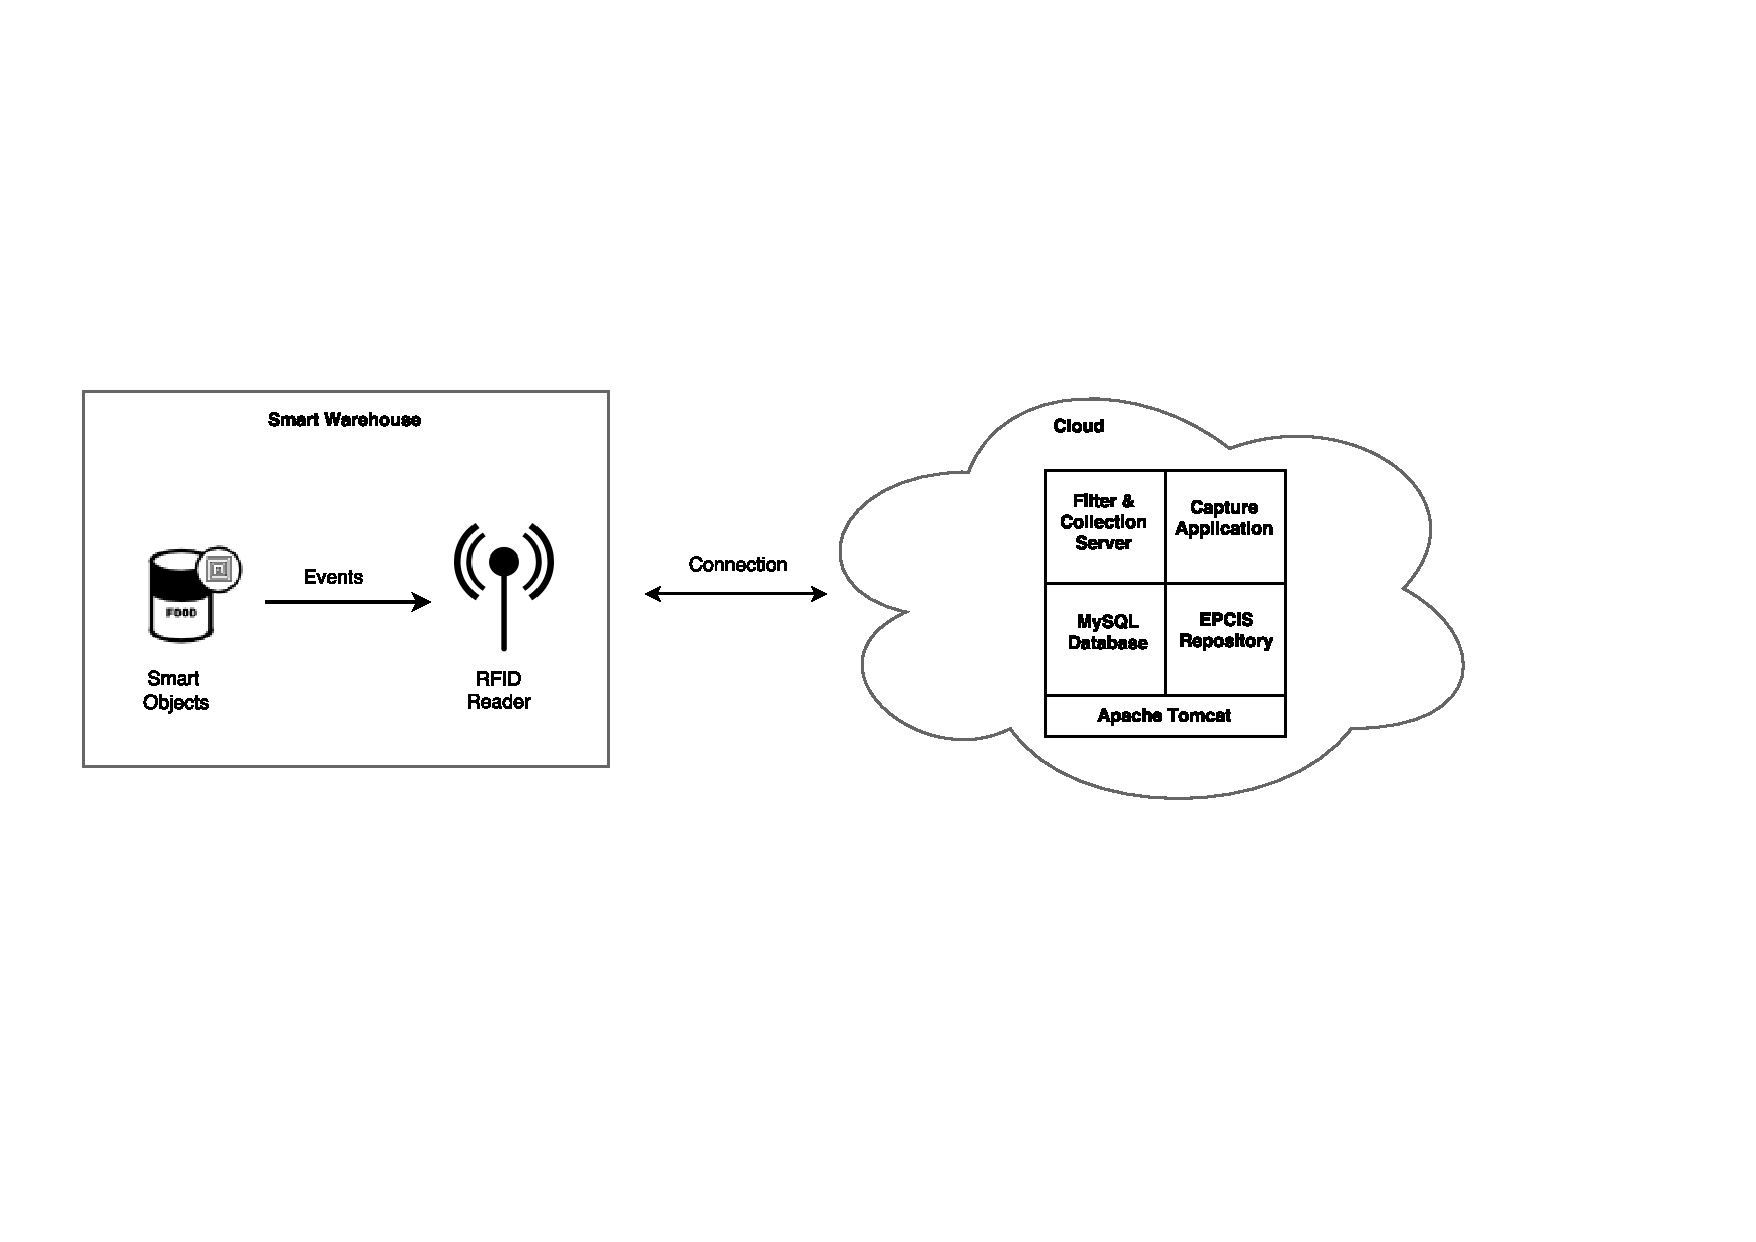
\includegraphics[width=\textwidth]{./images/implementation_cloud_architecture}
  \caption[Cloud-approach: technological architecture.]{Cloud-approach: smart warehouse technological architecture.}
  \label{fig:implementation_cloud_architecture}
\end{figure}

The \gls{RFID} middleware is provisioned in the cloud in a single virtual machine. In the
Fosstrak implementation the \gls{FCServer}, \gls{EPCIS} repository and the Capture application
requires an Apache servlet container to deploy and run the web applications. The \gls{EPCIS}
repository is connected to a MySQL database that stores the event data. The technological architecture
for the cloud approach is presented in Figure~\ref{fig:implementation_cloud_architecture}.\\

The smart warehouse can be connected to the cloud through a physical (e.g. \gls{ADSL} or Fiber-optic)
to a wireless connection (e.g. Wi-Fi, 3G or \gls{LTE}).

% Fog approach
\subsection{Fog Deployment}
\label{sub:imp_smart_warehouse_fog}

% Fog approach
\begin{figure}
  \centering
  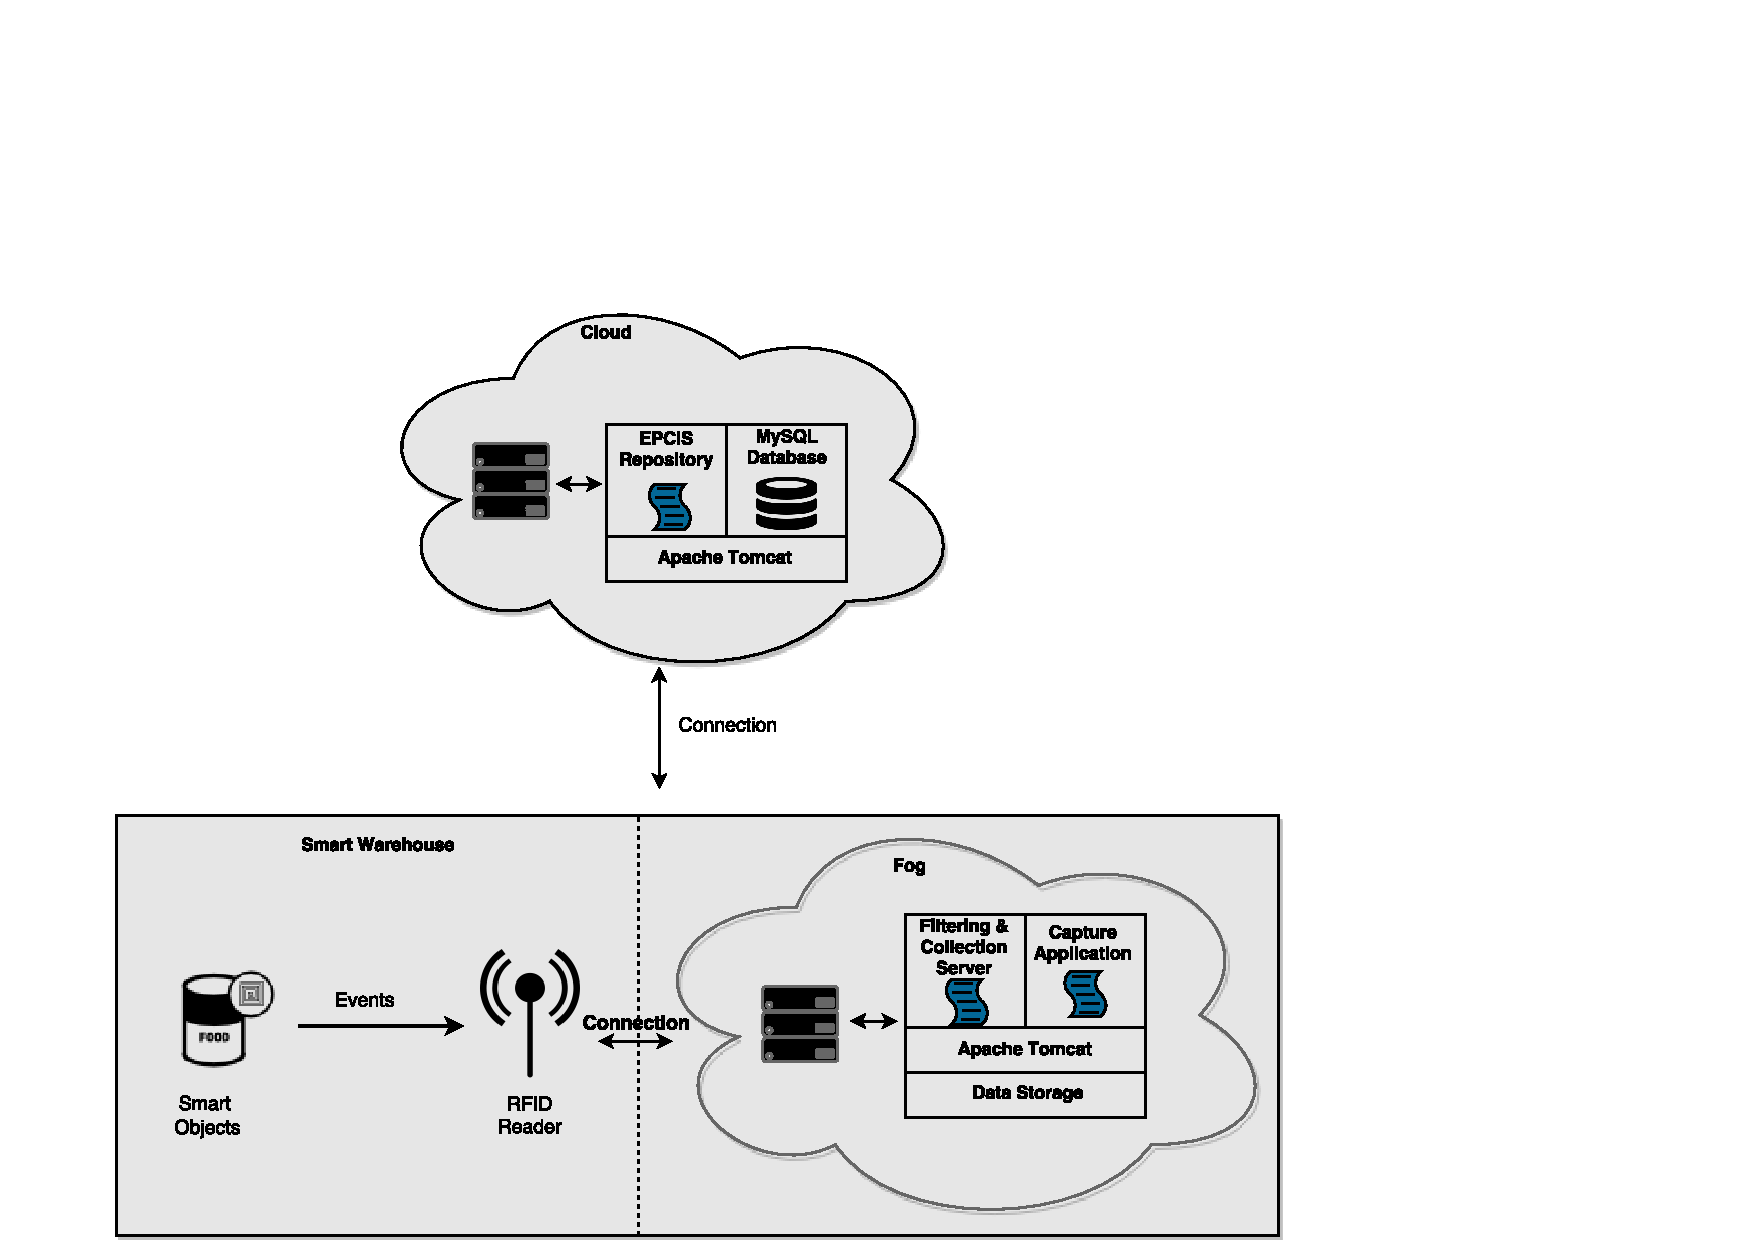
\includegraphics[width=\textwidth]{./images/implementation_fog_architecture}
  \caption[Fog-approach: technological architecture.]{Fog-approach: smart warehouse technological architecture.}
  \label{fig:implementation_fog_architecture}
\end{figure}

The \gls{RFID} middleware is provisioned across the fog and the cloud. At the cloud,
all the software components are provisioned in a single \gls{VM}. The \gls{EPCIS} repository is deployed
and running on top of an Apache Tomcat servlet instance. The repository is connected to a MySQL
database, which stores the event data. In the current implementation the fog was built with a traditional
\gls{VM}. The \gls{FCServer} and the Capture application are deployed and running on top of a single
Tomcat servlet instance. The Capture application sent the events collected by the \gls{FCServer} to
the \gls{EPCIS} repository through the \textit{\gls{EPCIS} Capture Interface} - via \gls{HTTP} requests.
Figure~\ref{fig:implementation_fog_architecture} presents the technological architecture for the fog
approach.\\

Both the smart warehouse as the fog can be connected respectively to the fog and cloud through several
types of connection, from a physical connection (e.g. \gls{ADSL} or Fiber-optic) to a wireless connection
(e.g. Wi-Fi, 3G or \gls{LTE}).

\section{Provisioning}
\label{sec:provisioning}
The implementation of the provisioning mechanism relies on the Chef tool. The recipes that describe our
infrastructure are based on cookbooks available at the Chef Supermarket\footnote{\url{https://supermarket.chef.io/}}.
These recipes describe how the Fosstrak software stack is provisioned in the cloud. In the current implementation,
we used Docker containers to provisioning the smart warehouse software at the cloud providers. To provisioning
the resources in the cloud instances we will use \textit{knife}, a command-line tool developed by
Chef that provides an interface between the local Chef repository and the Chef server. The provisioning
workflow is illustrated in Figure~\ref{fig:provisioning_tech_architecture}.\\

% Automatic provisioning diagram
\begin{figure}
  \centering
  \makebox[\textwidth][c]{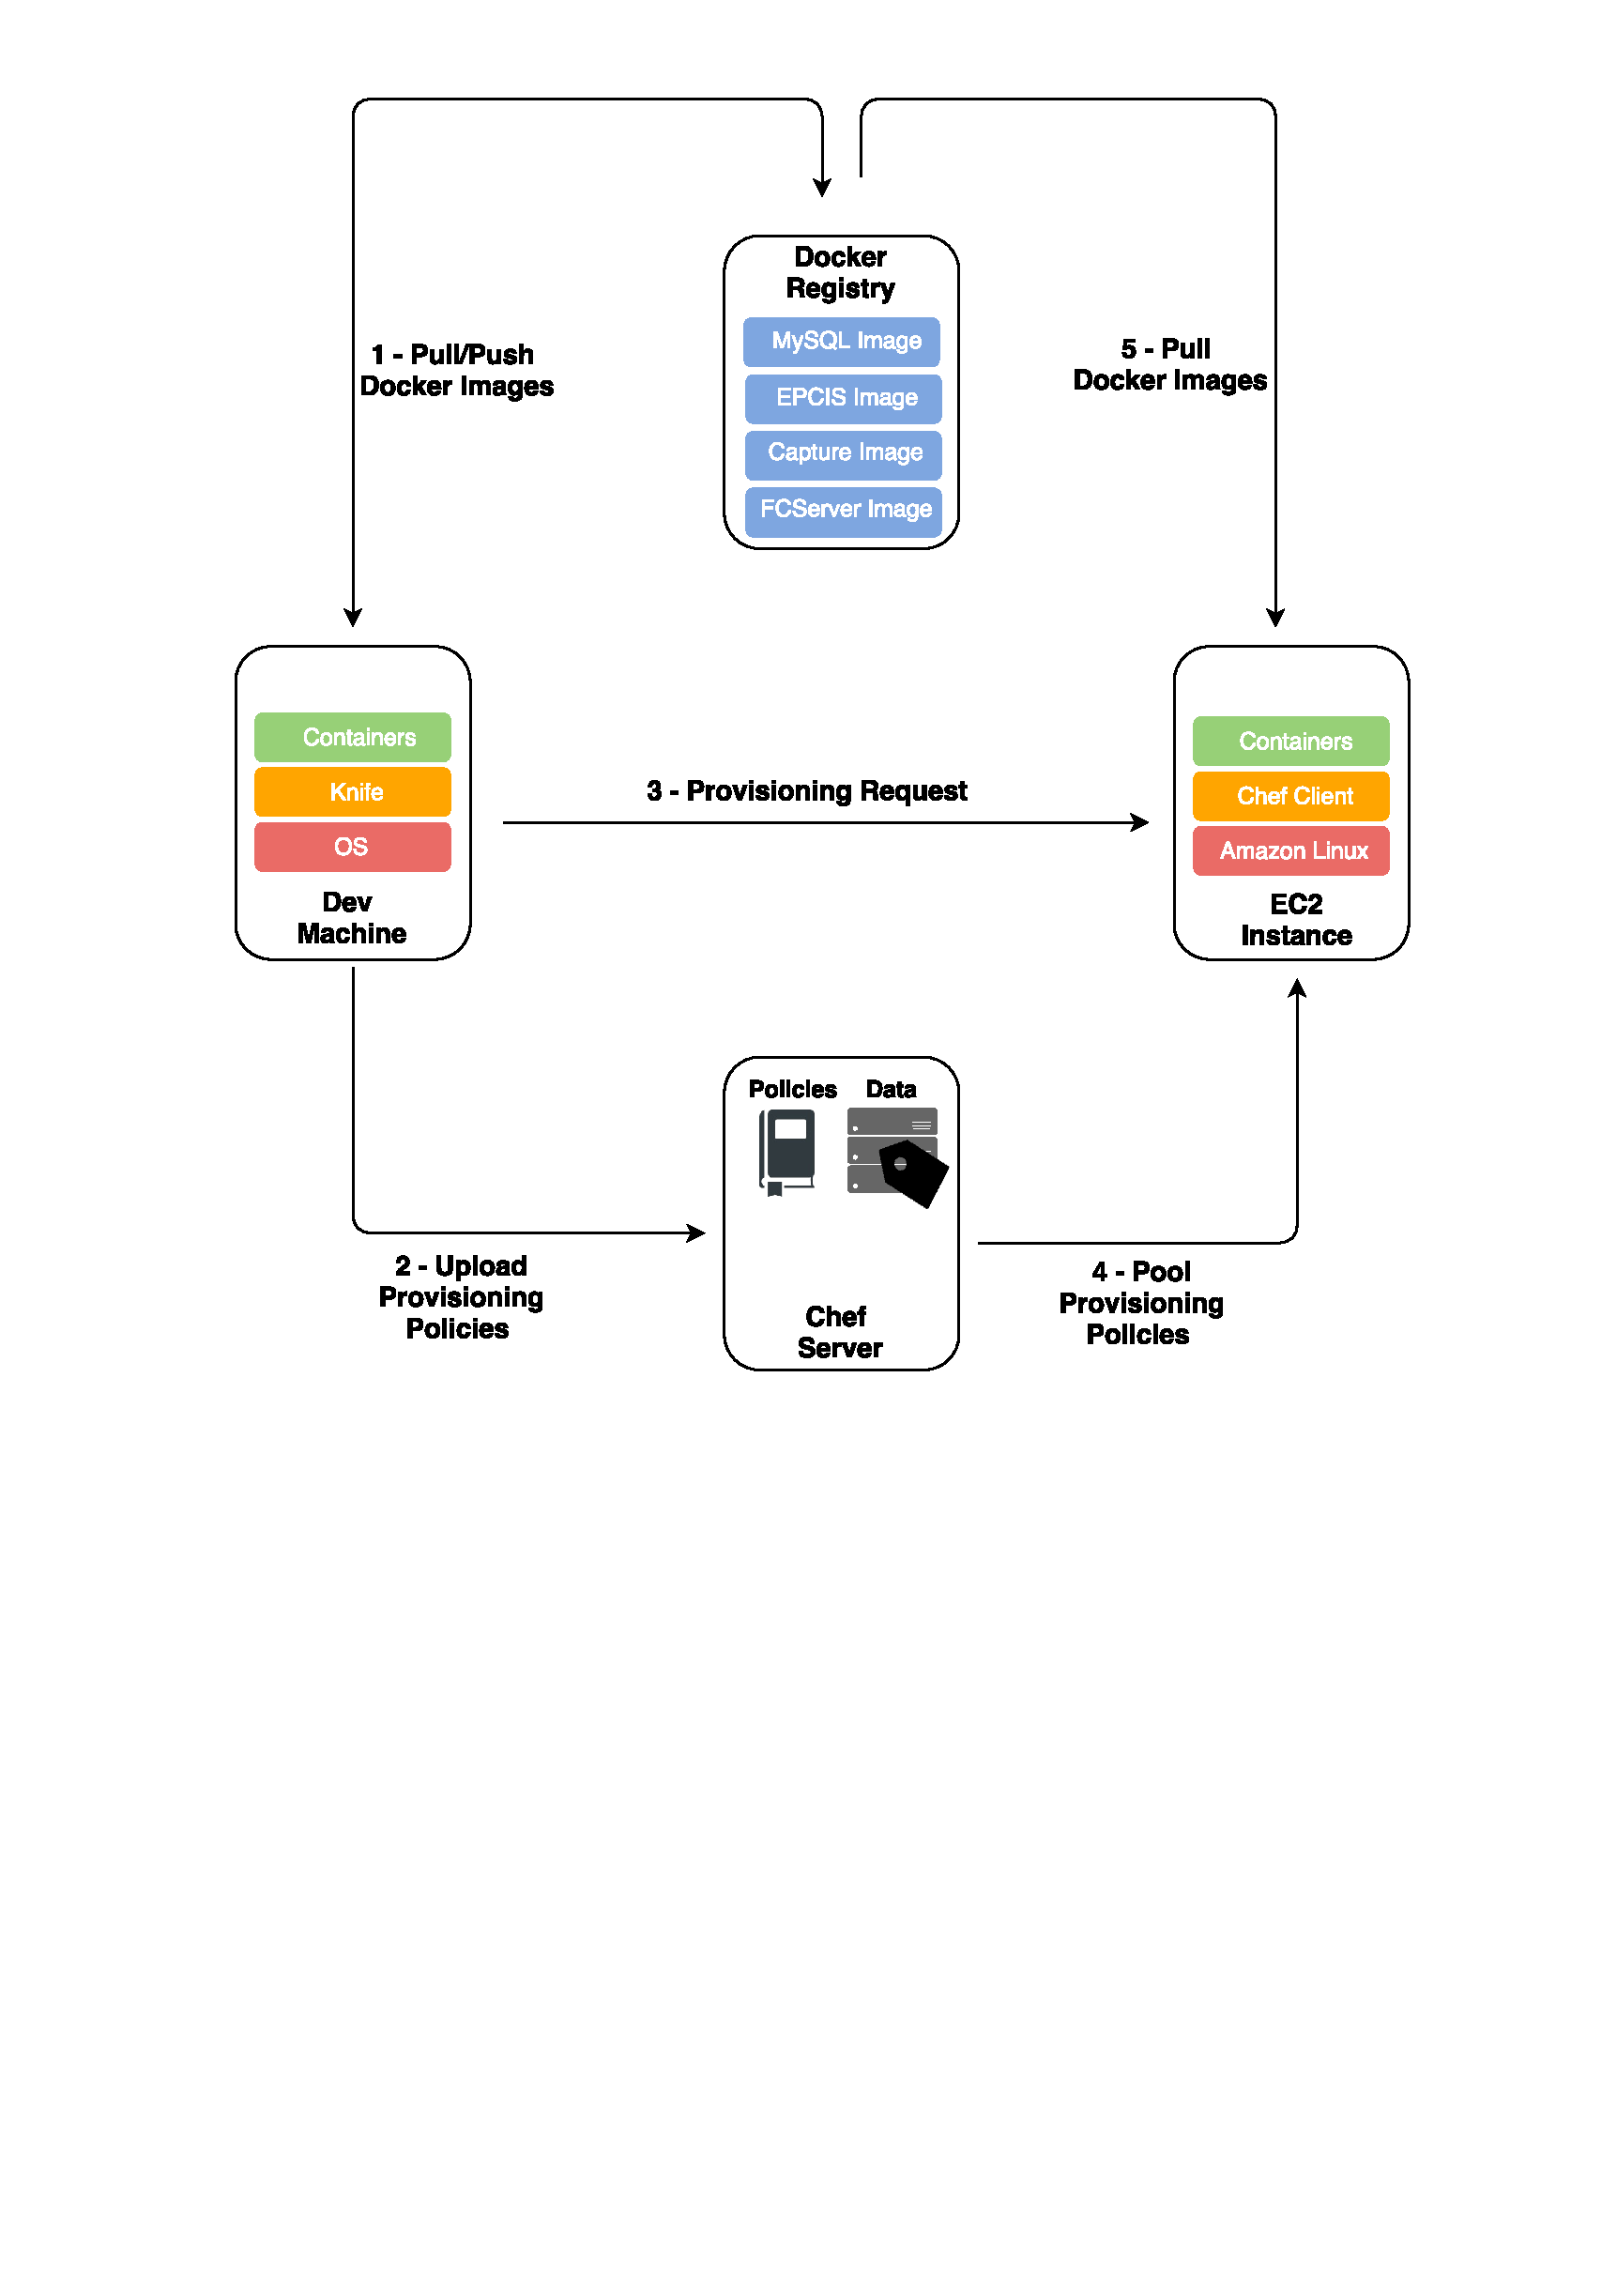
\includegraphics[width=.8\textwidth]{./images/c4t-tech-architecture}}%
  \caption[Automatic provisioning workflow.]{Automatic provisioning workflow.}
  \label{fig:provisioning_tech_architecture}
\end{figure}

In a development environment the Docker images are built and then uploaded to the Docker Registry
repository (1). The provisioning of the cloud resources is described in the cookbooks that are uploaded
to the Chef server (2). The provisioning request (3) is performed using \textit{knife}, that allows to
describe the image type, the instance type and the policies that need to be applied on each provisioned node.
Then the Chef client runs the configuration recipes that are pulled from the Chef server (4). In our
solution these configuration recipes describe that our nodes must have a set of Docker containers
running on it. The Chef client pulls the Docker images from the remote repository, build the containers
based on those images and finally applies the configuration that is associated to each container.\\

We decide to chose Chef instead of its competitors - i.e. Puppet and Ansible - for several
reasons, where the main one is \textit{knife}. \textit{Knife} is very powerful and allow us to
interact with our entire infrastructure. For instance, it is possible to bootstrap a new server,
apply a role to a set of nodes in our environment. Furthermore, with \textit{knife ssh} it is
possible to execute a command on a certain number of nodes in our environment.

% Docker containers
\subsection{Docker Containers}
\label{sub:impl_docker}
Docker containers are used to provisioning the software stack of the Fosstrak platform. A complete
installation of Fosstrak requires a compatible Java \gls{SDK}, a full MySQL database and a Apache Tomcat
server.\\

As illustrated in Figure~\ref{fig:impl_containers}, we are provisioning a single container for each
component of the Fosstrak platform, the \gls{EPCIS} repository, the Capture application, the \gls{FCServer},
and also for the MySQL database. In our implementation, the container images of the Fosstrak stack
are published in the Docker Hub repository to later be used to create the containers.\\

% Container stack
\begin{figure}[!ht]
  \centering
  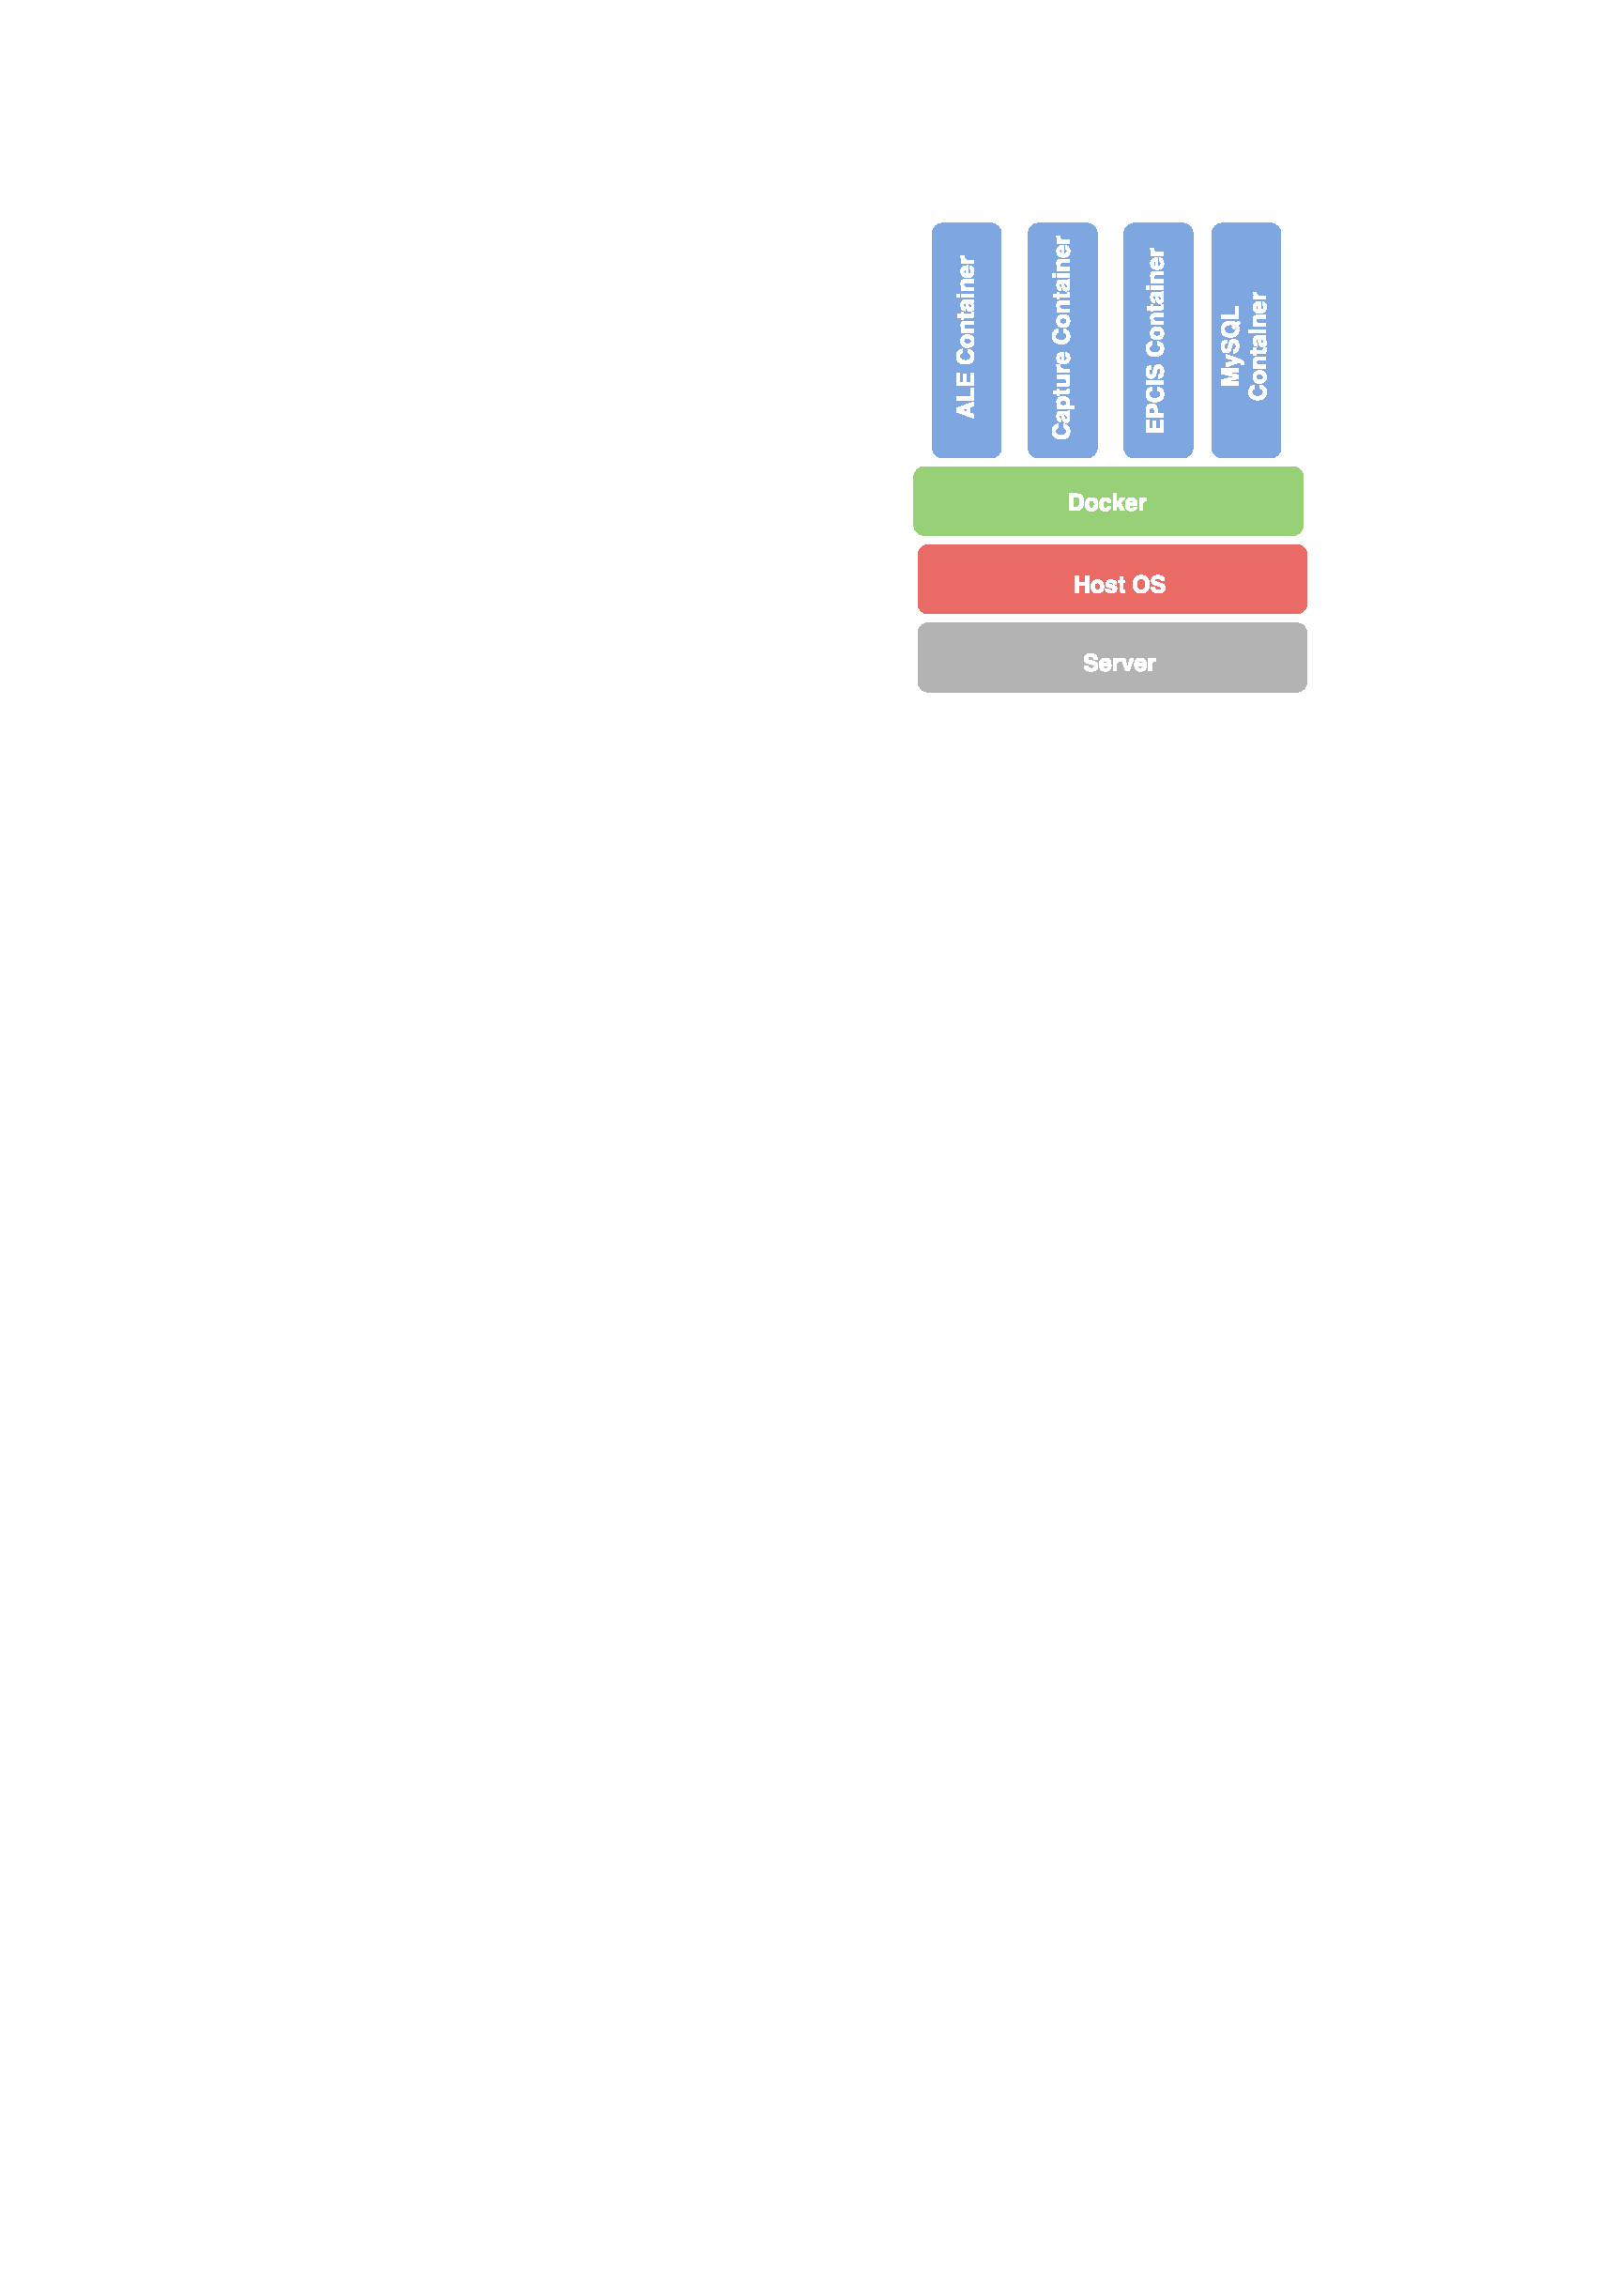
\includegraphics[width=.3\textwidth]{./images/docker-stack}
  \caption[Fosstrak containers stack.]{Fosstrak containers stack.}
  \label{fig:impl_containers}
\end{figure}

By default each container runs a process that is isolated from the other processes that are executed
in the same environment. In order to connect the different modules of the Fosstrak, our containers are
linked through the \textit{linking system} provided by Docker. This mechanism creates a secure tunnel
between the containers, allowing the recipient container to access selected data about the source container.
For instance, our \gls{EPCIS} container - which is linked to the MySQL database container - is able to
access information about the MySQL container.\\

The reasons that we chose Docker containers instead of traditional \glspl{VM} is that containers are a
virtualization platform which its images requires less disk space and I/O when compared with traditional
\gls{VM} images \cite{merkel2014docker}. Furthermore, Docker containers are portable, which means that
they can be moved across different infrastructures depending on how the application scales.
